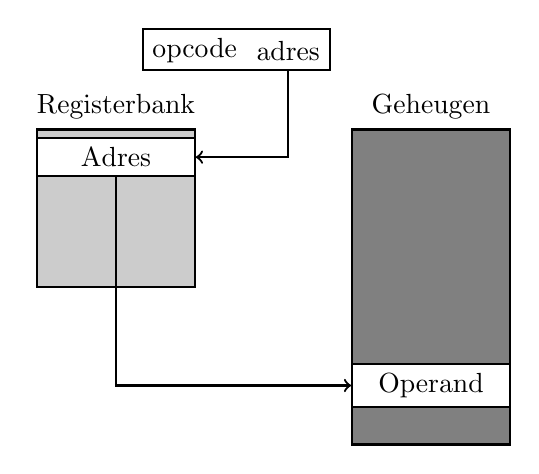
\begin{tikzpicture}
\node (IA) at (0,0) {opcode};
\node[anchor=west] (IB) at (IA.east) {adres};
\draw[thick] (IA.north west) rectangle (IB.south east);
\begin{scope}[xshift=3cm,yshift=-3cm]
\node[draw,rectangle,thick,fill=gray,minimum width=2 cm,minimum height=4 cm] (MEM) at (0,0) {};
\node[draw,rectangle,thick,fill=white,minimum width=2 cm] (OPE) at (0,-1.25) {Operand};
\draw (MEM.north) node[anchor=south] {Geheugen};
\end{scope}
\begin{scope}[xshift=-1cm,yshift=-2cm]
\node[draw,rectangle,thick,fill=black!20!white,minimum width=2 cm,minimum height=2 cm] (RGB) at (0,0) {};
\node[draw,rectangle,thick,fill=white,minimum width=2 cm] (ADR) at (0,0.65) {Adres};
\draw (RGB.north) node[anchor=south] {Registerbank};
\end{scope}
\draw[thick,->] (IB) |- (ADR);
\draw[thick,->] (ADR) |- (OPE);
\end{tikzpicture}